\documentclass[12pt,a4paper]{article}
\usepackage{a4wide}
\usepackage[T1]{fontenc}
\usepackage[utf8]{inputenc}
\usepackage[czech]{babel}
\usepackage{amsmath, amsfonts, amssymb}
\usepackage{graphicx}

\addtolength{\voffset}{-1cm}
\addtolength{\textheight}{3cm}
\addtolength{\headheight}{2cm}
\addtolength{\headsep}{-3cm}

\begin{document}

%   ť   Ť

\setlength{\parskip}{0.2cm}
\setlength{\parindent}{0cm}

\section{Písmenka}

Aaaaaa

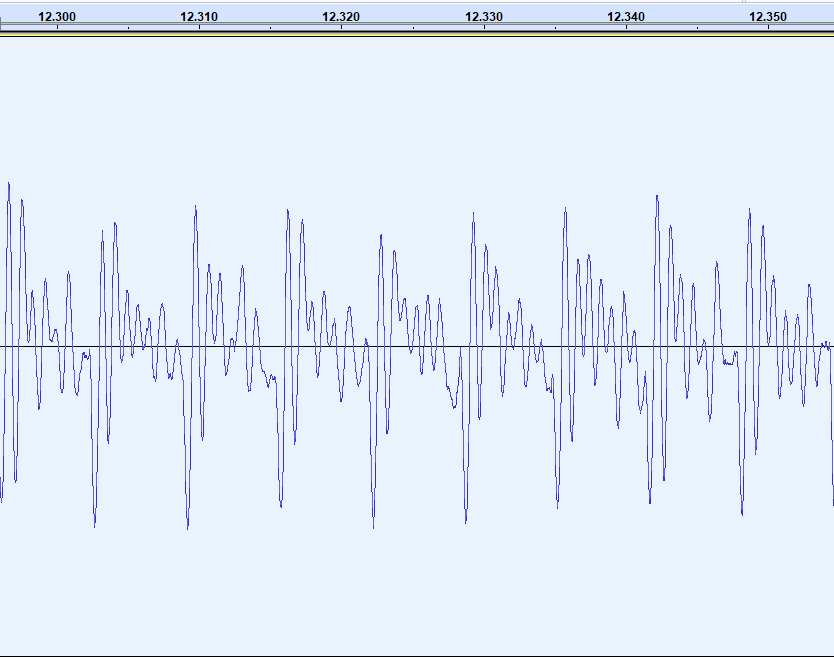
\includegraphics[height=5cm,width=10cm]{aaa.png}

Eeeeee

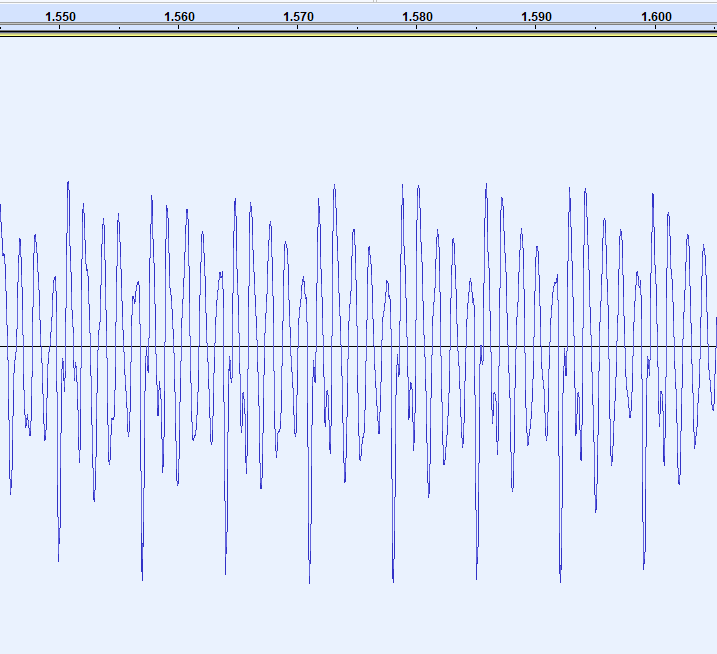
\includegraphics[height=5cm,width=10cm]{eee.png}

Uuuuu

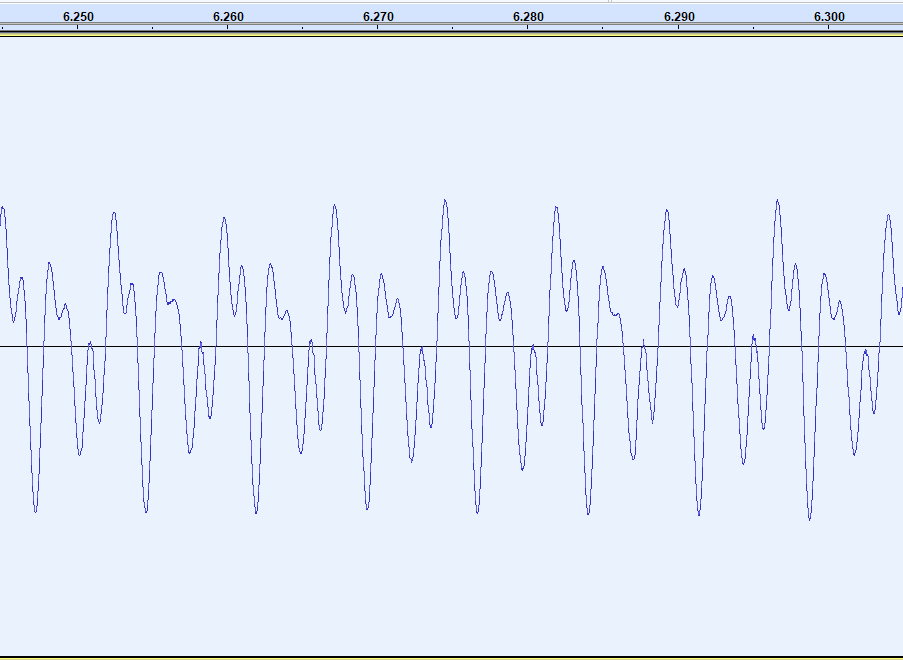
\includegraphics[height=5cm,width=10cm]{uuu.png}

\newpage

\section{A od všech}

Jirka

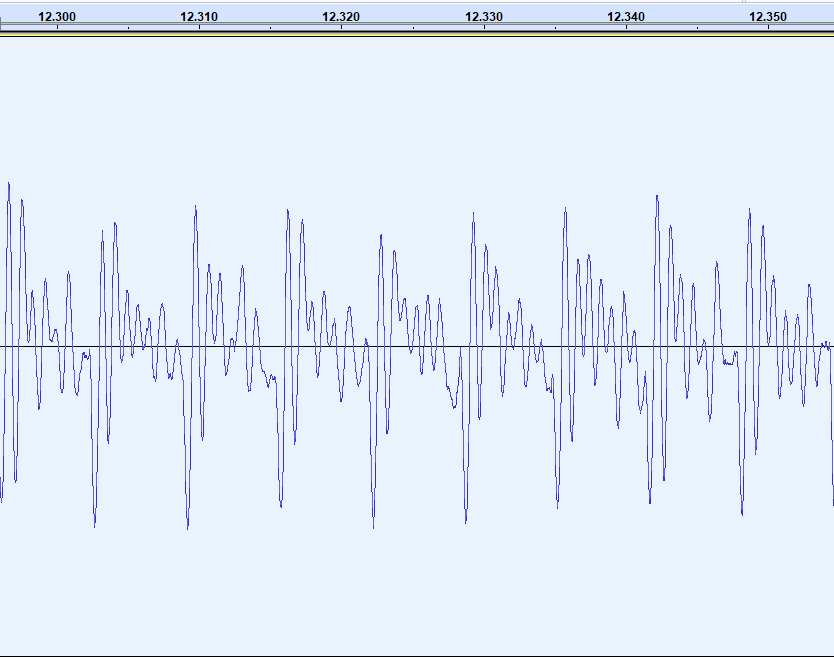
\includegraphics[height=5cm,width=10cm]{aaa.png}

Jindra

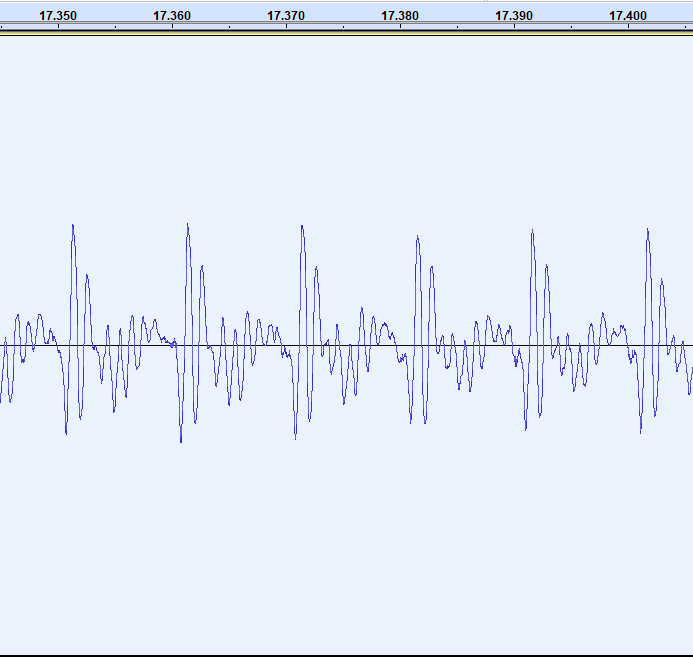
\includegraphics[height=5cm,width=10cm]{aaaj.png}

Klára

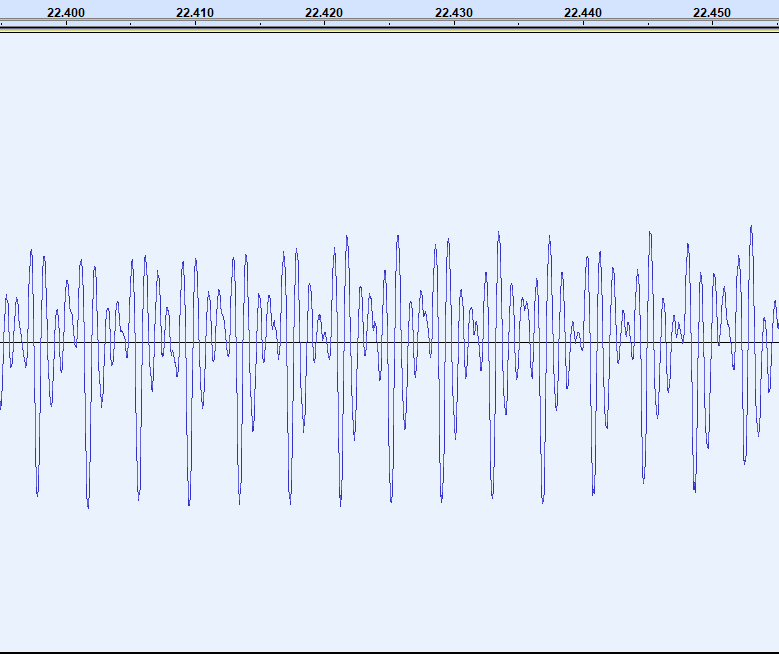
\includegraphics[height=5cm,width=10cm]{aaak.png}

\newpage

\section{Rozsah frekvencí}

Jindra

\def\f{\frac}
Nejnižší - $\f{1}{0.009}\ {\rm s^{-1}}$\\
Nejvyšší - $\f{15}{0.014}\ {\rm s^{-1}}$

Jirka

Nejnižší - $\f{1}{0.010}\ {\rm s^{-1}}$\\
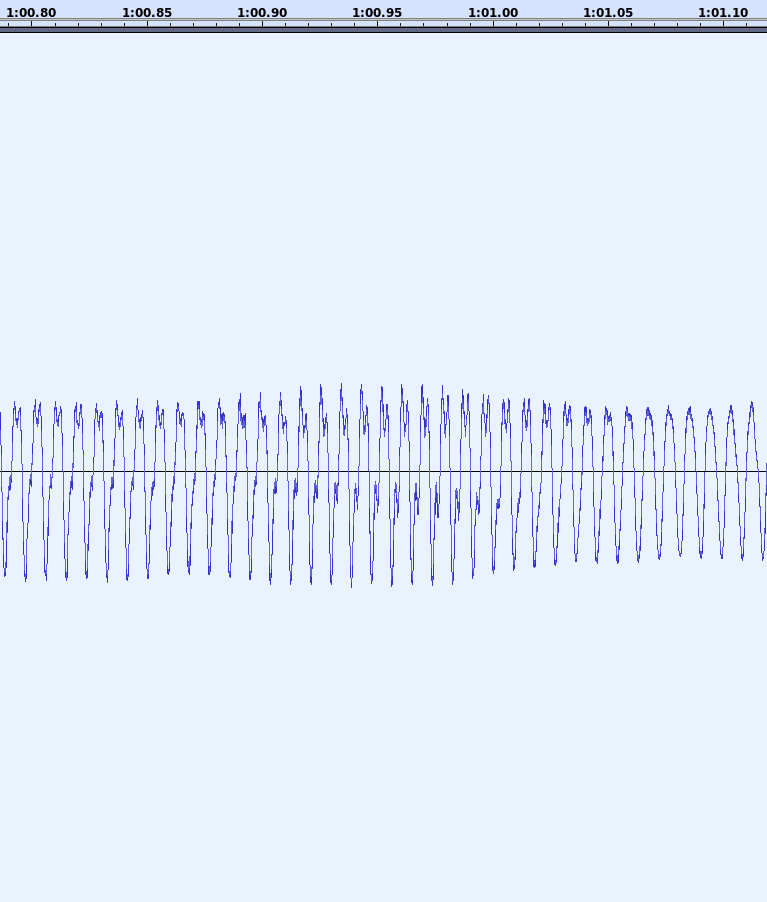
\includegraphics[height=5cm,width=10cm]{min.png}\\
Nejvyšší - $\f{1}{0.002}\ {\rm s^{-1}}$\\
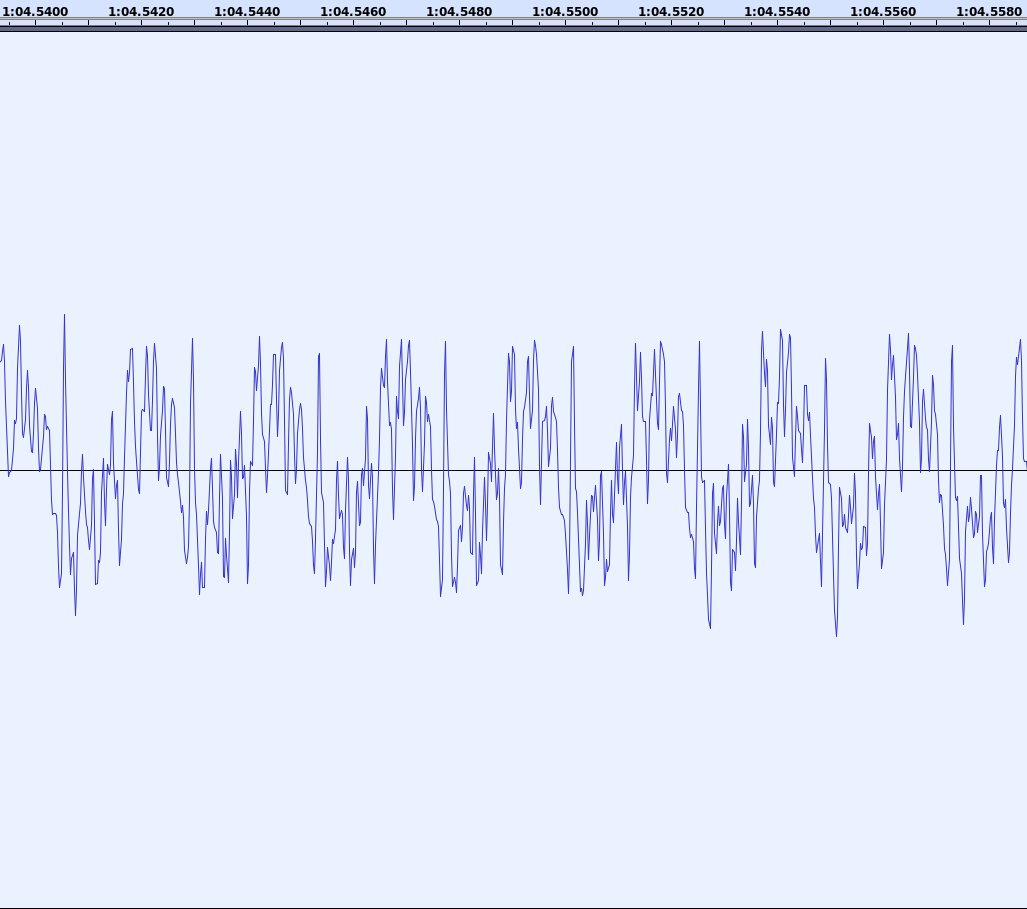
\includegraphics[height=5cm,width=10cm]{max.png}

\newpage
\section{Ladička}
Ladičku bohužel doma nemám a v hodině jsme zaznamenali pouze rázy:\\
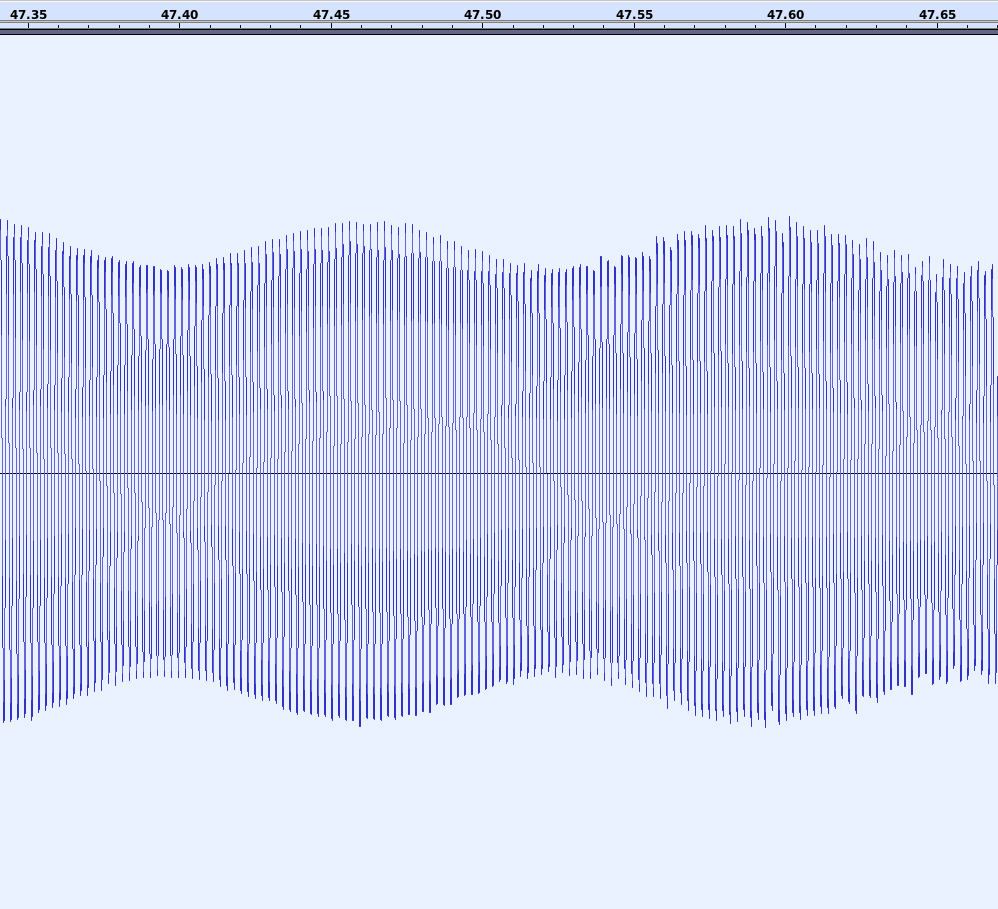
\includegraphics[height=5cm,width=10cm]{ladicka.png}

Frekvence rázů je - $\f{1}{0.124}\ {\rm s^{-1}}$
\section{Snižování frekvence}
Zvuk přestává být srozumitelný, vyšší frekvence se ztrácí, nakonec není slyšet nic.

\section{Otázky}
\begin{enumerate}
	\item Posun membrány vůči původní poloze.
	\item Na vstupu dostane analogový signál (např. zvuk) a na výstup ho popisuje digitálně, tak aby se dal zpracovat další elektronikou (procesorem).
	\item Vzorkovací frekvence -- počet záznamů zvuku za sekundu; rozsah -- počet hodnot, které jsme schopni rozlišit u každého záznamu (resp. logaritmus této hodnoty).
	\item $10\ 584\ 000 B$.
\end{enumerate}



\end{document}
